% Options for packages loaded elsewhere
\PassOptionsToPackage{unicode}{hyperref}
\PassOptionsToPackage{hyphens}{url}
\PassOptionsToPackage{dvipsnames,svgnames,x11names}{xcolor}
%
\documentclass[
  letterpaper,
  DIV=11,
  numbers=noendperiod]{scrartcl}

\usepackage{amsmath,amssymb}
\usepackage{iftex}
\ifPDFTeX
  \usepackage[T1]{fontenc}
  \usepackage[utf8]{inputenc}
  \usepackage{textcomp} % provide euro and other symbols
\else % if luatex or xetex
  \usepackage{unicode-math}
  \defaultfontfeatures{Scale=MatchLowercase}
  \defaultfontfeatures[\rmfamily]{Ligatures=TeX,Scale=1}
\fi
\usepackage{lmodern}
\ifPDFTeX\else  
    % xetex/luatex font selection
\fi
% Use upquote if available, for straight quotes in verbatim environments
\IfFileExists{upquote.sty}{\usepackage{upquote}}{}
\IfFileExists{microtype.sty}{% use microtype if available
  \usepackage[]{microtype}
  \UseMicrotypeSet[protrusion]{basicmath} % disable protrusion for tt fonts
}{}
\makeatletter
\@ifundefined{KOMAClassName}{% if non-KOMA class
  \IfFileExists{parskip.sty}{%
    \usepackage{parskip}
  }{% else
    \setlength{\parindent}{0pt}
    \setlength{\parskip}{6pt plus 2pt minus 1pt}}
}{% if KOMA class
  \KOMAoptions{parskip=half}}
\makeatother
\usepackage{xcolor}
\setlength{\emergencystretch}{3em} % prevent overfull lines
\setcounter{secnumdepth}{-\maxdimen} % remove section numbering
% Make \paragraph and \subparagraph free-standing
\ifx\paragraph\undefined\else
  \let\oldparagraph\paragraph
  \renewcommand{\paragraph}[1]{\oldparagraph{#1}\mbox{}}
\fi
\ifx\subparagraph\undefined\else
  \let\oldsubparagraph\subparagraph
  \renewcommand{\subparagraph}[1]{\oldsubparagraph{#1}\mbox{}}
\fi

\usepackage{color}
\usepackage{fancyvrb}
\newcommand{\VerbBar}{|}
\newcommand{\VERB}{\Verb[commandchars=\\\{\}]}
\DefineVerbatimEnvironment{Highlighting}{Verbatim}{commandchars=\\\{\}}
% Add ',fontsize=\small' for more characters per line
\usepackage{framed}
\definecolor{shadecolor}{RGB}{241,243,245}
\newenvironment{Shaded}{\begin{snugshade}}{\end{snugshade}}
\newcommand{\AlertTok}[1]{\textcolor[rgb]{0.68,0.00,0.00}{#1}}
\newcommand{\AnnotationTok}[1]{\textcolor[rgb]{0.37,0.37,0.37}{#1}}
\newcommand{\AttributeTok}[1]{\textcolor[rgb]{0.40,0.45,0.13}{#1}}
\newcommand{\BaseNTok}[1]{\textcolor[rgb]{0.68,0.00,0.00}{#1}}
\newcommand{\BuiltInTok}[1]{\textcolor[rgb]{0.00,0.23,0.31}{#1}}
\newcommand{\CharTok}[1]{\textcolor[rgb]{0.13,0.47,0.30}{#1}}
\newcommand{\CommentTok}[1]{\textcolor[rgb]{0.37,0.37,0.37}{#1}}
\newcommand{\CommentVarTok}[1]{\textcolor[rgb]{0.37,0.37,0.37}{\textit{#1}}}
\newcommand{\ConstantTok}[1]{\textcolor[rgb]{0.56,0.35,0.01}{#1}}
\newcommand{\ControlFlowTok}[1]{\textcolor[rgb]{0.00,0.23,0.31}{#1}}
\newcommand{\DataTypeTok}[1]{\textcolor[rgb]{0.68,0.00,0.00}{#1}}
\newcommand{\DecValTok}[1]{\textcolor[rgb]{0.68,0.00,0.00}{#1}}
\newcommand{\DocumentationTok}[1]{\textcolor[rgb]{0.37,0.37,0.37}{\textit{#1}}}
\newcommand{\ErrorTok}[1]{\textcolor[rgb]{0.68,0.00,0.00}{#1}}
\newcommand{\ExtensionTok}[1]{\textcolor[rgb]{0.00,0.23,0.31}{#1}}
\newcommand{\FloatTok}[1]{\textcolor[rgb]{0.68,0.00,0.00}{#1}}
\newcommand{\FunctionTok}[1]{\textcolor[rgb]{0.28,0.35,0.67}{#1}}
\newcommand{\ImportTok}[1]{\textcolor[rgb]{0.00,0.46,0.62}{#1}}
\newcommand{\InformationTok}[1]{\textcolor[rgb]{0.37,0.37,0.37}{#1}}
\newcommand{\KeywordTok}[1]{\textcolor[rgb]{0.00,0.23,0.31}{#1}}
\newcommand{\NormalTok}[1]{\textcolor[rgb]{0.00,0.23,0.31}{#1}}
\newcommand{\OperatorTok}[1]{\textcolor[rgb]{0.37,0.37,0.37}{#1}}
\newcommand{\OtherTok}[1]{\textcolor[rgb]{0.00,0.23,0.31}{#1}}
\newcommand{\PreprocessorTok}[1]{\textcolor[rgb]{0.68,0.00,0.00}{#1}}
\newcommand{\RegionMarkerTok}[1]{\textcolor[rgb]{0.00,0.23,0.31}{#1}}
\newcommand{\SpecialCharTok}[1]{\textcolor[rgb]{0.37,0.37,0.37}{#1}}
\newcommand{\SpecialStringTok}[1]{\textcolor[rgb]{0.13,0.47,0.30}{#1}}
\newcommand{\StringTok}[1]{\textcolor[rgb]{0.13,0.47,0.30}{#1}}
\newcommand{\VariableTok}[1]{\textcolor[rgb]{0.07,0.07,0.07}{#1}}
\newcommand{\VerbatimStringTok}[1]{\textcolor[rgb]{0.13,0.47,0.30}{#1}}
\newcommand{\WarningTok}[1]{\textcolor[rgb]{0.37,0.37,0.37}{\textit{#1}}}

\providecommand{\tightlist}{%
  \setlength{\itemsep}{0pt}\setlength{\parskip}{0pt}}\usepackage{longtable,booktabs,array}
\usepackage{calc} % for calculating minipage widths
% Correct order of tables after \paragraph or \subparagraph
\usepackage{etoolbox}
\makeatletter
\patchcmd\longtable{\par}{\if@noskipsec\mbox{}\fi\par}{}{}
\makeatother
% Allow footnotes in longtable head/foot
\IfFileExists{footnotehyper.sty}{\usepackage{footnotehyper}}{\usepackage{footnote}}
\makesavenoteenv{longtable}
\usepackage{graphicx}
\makeatletter
\def\maxwidth{\ifdim\Gin@nat@width>\linewidth\linewidth\else\Gin@nat@width\fi}
\def\maxheight{\ifdim\Gin@nat@height>\textheight\textheight\else\Gin@nat@height\fi}
\makeatother
% Scale images if necessary, so that they will not overflow the page
% margins by default, and it is still possible to overwrite the defaults
% using explicit options in \includegraphics[width, height, ...]{}
\setkeys{Gin}{width=\maxwidth,height=\maxheight,keepaspectratio}
% Set default figure placement to htbp
\makeatletter
\def\fps@figure{htbp}
\makeatother

\KOMAoption{captions}{tableheading}
\makeatletter
\@ifpackageloaded{tcolorbox}{}{\usepackage[skins,breakable]{tcolorbox}}
\@ifpackageloaded{fontawesome5}{}{\usepackage{fontawesome5}}
\definecolor{quarto-callout-color}{HTML}{909090}
\definecolor{quarto-callout-note-color}{HTML}{0758E5}
\definecolor{quarto-callout-important-color}{HTML}{CC1914}
\definecolor{quarto-callout-warning-color}{HTML}{EB9113}
\definecolor{quarto-callout-tip-color}{HTML}{00A047}
\definecolor{quarto-callout-caution-color}{HTML}{FC5300}
\definecolor{quarto-callout-color-frame}{HTML}{acacac}
\definecolor{quarto-callout-note-color-frame}{HTML}{4582ec}
\definecolor{quarto-callout-important-color-frame}{HTML}{d9534f}
\definecolor{quarto-callout-warning-color-frame}{HTML}{f0ad4e}
\definecolor{quarto-callout-tip-color-frame}{HTML}{02b875}
\definecolor{quarto-callout-caution-color-frame}{HTML}{fd7e14}
\makeatother
\makeatletter
\@ifpackageloaded{caption}{}{\usepackage{caption}}
\AtBeginDocument{%
\ifdefined\contentsname
  \renewcommand*\contentsname{Table of contents}
\else
  \newcommand\contentsname{Table of contents}
\fi
\ifdefined\listfigurename
  \renewcommand*\listfigurename{List of Figures}
\else
  \newcommand\listfigurename{List of Figures}
\fi
\ifdefined\listtablename
  \renewcommand*\listtablename{List of Tables}
\else
  \newcommand\listtablename{List of Tables}
\fi
\ifdefined\figurename
  \renewcommand*\figurename{Figure}
\else
  \newcommand\figurename{Figure}
\fi
\ifdefined\tablename
  \renewcommand*\tablename{Table}
\else
  \newcommand\tablename{Table}
\fi
}
\@ifpackageloaded{float}{}{\usepackage{float}}
\floatstyle{ruled}
\@ifundefined{c@chapter}{\newfloat{codelisting}{h}{lop}}{\newfloat{codelisting}{h}{lop}[chapter]}
\floatname{codelisting}{Listing}
\newcommand*\listoflistings{\listof{codelisting}{List of Listings}}
\makeatother
\makeatletter
\makeatother
\makeatletter
\@ifpackageloaded{caption}{}{\usepackage{caption}}
\@ifpackageloaded{subcaption}{}{\usepackage{subcaption}}
\makeatother
\ifLuaTeX
  \usepackage{selnolig}  % disable illegal ligatures
\fi
\usepackage{bookmark}

\IfFileExists{xurl.sty}{\usepackage{xurl}}{} % add URL line breaks if available
\urlstyle{same} % disable monospaced font for URLs
\hypersetup{
  pdftitle={Homework 6},
  pdfauthor={Matt Viana},
  colorlinks=true,
  linkcolor={blue},
  filecolor={Maroon},
  citecolor={Blue},
  urlcolor={Blue},
  pdfcreator={LaTeX via pandoc}}

\title{Homework 6}
\author{{Matt Viana}}
\date{}

\begin{document}
\maketitle

\renewcommand*\contentsname{Table of contents}
{
\hypersetup{linkcolor=}
\setcounter{tocdepth}{3}
\tableofcontents
}
\begin{tcolorbox}[enhanced jigsaw, leftrule=.75mm, rightrule=.15mm, left=2mm, colframe=quarto-callout-important-color-frame, bottomtitle=1mm, colbacktitle=quarto-callout-important-color!10!white, titlerule=0mm, breakable, opacitybacktitle=0.6, coltitle=black, arc=.35mm, colback=white, title=\textcolor{quarto-callout-important-color}{\faExclamation}\hspace{0.5em}{Important}, toptitle=1mm, toprule=.15mm, bottomrule=.15mm, opacityback=0]

Please read the instructions carefully before submitting your
assignment.

\begin{enumerate}
\def\labelenumi{\arabic{enumi}.}
\tightlist
\item
  This assignment requires you to only upload a \texttt{PDF} file on
  Canvas
\item
  Don't collapse any code cells before submitting.
\item
  Remember to make sure all your code output is rendered properly before
  uploading your submission.
\end{enumerate}

⚠️ Please add your name to the author information in the frontmatter
before submitting your assignment ⚠️

\end{tcolorbox}

In this assignment, we will perform various tasks involving principal
component analysis (PCA), principal component regression, and
dimensionality reduction.

We will need the following packages:

\begin{Shaded}
\begin{Highlighting}[]
\NormalTok{packages }\OtherTok{\textless{}{-}} \FunctionTok{c}\NormalTok{(}
  \StringTok{"tibble"}\NormalTok{,}
  \StringTok{"dplyr"}\NormalTok{, }
  \StringTok{"readr"}\NormalTok{, }
  \StringTok{"tidyr"}\NormalTok{, }
  \StringTok{"purrr"}\NormalTok{, }
  \StringTok{"broom"}\NormalTok{,}
  \StringTok{"magrittr"}\NormalTok{,}
  \StringTok{"corrplot"}\NormalTok{,}
  \StringTok{"car"}\NormalTok{,}
  \StringTok{"janitor"}\NormalTok{,}
  \StringTok{"ggplot2"}\NormalTok{,}
  \StringTok{"reshape2"}
\NormalTok{)}
\CommentTok{\# renv::install(packages)}
\FunctionTok{sapply}\NormalTok{(packages, require, }\AttributeTok{character.only=}\NormalTok{T)}
\end{Highlighting}
\end{Shaded}

\subsection{\texorpdfstring{}{ }}\label{section}

\subsection{Question 1}\label{question-1}

\begin{tcolorbox}[enhanced jigsaw, leftrule=.75mm, rightrule=.15mm, left=2mm, colframe=quarto-callout-tip-color-frame, bottomtitle=1mm, colbacktitle=quarto-callout-tip-color!10!white, titlerule=0mm, breakable, opacitybacktitle=0.6, coltitle=black, arc=.35mm, colback=white, title=\textcolor{quarto-callout-tip-color}{\faLightbulb}\hspace{0.5em}{70 points}, toptitle=1mm, toprule=.15mm, bottomrule=.15mm, opacityback=0]

Principal component anlaysis and variable selection

\end{tcolorbox}

1.1 (5 points)

The \texttt{data} folder contains a \texttt{spending.csv} dataset which
is an illustrative sample of monthly spending data for a group of
\(5000\) people across a variety of categories. The response variable,
\texttt{income}, is their monthly income, and objective is to predict
the \texttt{income} for a an individual based on their spending
patterns.

Read the data file as a tibble in R. Preprocess the data such that:

\begin{enumerate}
\def\labelenumi{\arabic{enumi}.}
\tightlist
\item
  the variables are of the right data type, e.g., categorical variables
  are encoded as factors
\item
  all column names to lower case for consistency
\item
  Any observations with missing values are dropped
\end{enumerate}

\begin{Shaded}
\begin{Highlighting}[]
\NormalTok{path }\OtherTok{\textless{}{-}} \StringTok{"data/spending.csv"}
\NormalTok{df }\OtherTok{\textless{}{-}} \FunctionTok{read\_csv}\NormalTok{(path) }\SpecialCharTok{\%\textgreater{}\%}
\NormalTok{  janitor}\SpecialCharTok{::}\FunctionTok{clean\_names}\NormalTok{() }\SpecialCharTok{\%\textgreater{}\%}
  \FunctionTok{mutate\_if}\NormalTok{(is.character, as.factor) }\SpecialCharTok{\%\textgreater{}\%}
  \FunctionTok{na.omit}\NormalTok{()}
\end{Highlighting}
\end{Shaded}

\begin{verbatim}
Rows: 5000 Columns: 40
-- Column specification --------------------------------------------------------
Delimiter: ","
dbl (40): accessories, accommodation, alcohol, audio_equipment, beverages, b...

i Use `spec()` to retrieve the full column specification for this data.
i Specify the column types or set `show_col_types = FALSE` to quiet this message.
\end{verbatim}

\begin{center}\rule{0.5\linewidth}{0.5pt}\end{center}

1.2 (5 points)

Visualize the correlation between the variables using the
\texttt{corrplot()} function. What do you observe? What does this mean
for the model?

\begin{Shaded}
\begin{Highlighting}[]
\NormalTok{df\_x }\OtherTok{\textless{}{-}}\NormalTok{ df }\SpecialCharTok{\%\textgreater{}\%}
  \FunctionTok{select}\NormalTok{(}\SpecialCharTok{{-}}\NormalTok{income) }\SpecialCharTok{\%\textgreater{}\%}
  \FunctionTok{cor}\NormalTok{() }\SpecialCharTok{\%\textgreater{}\%}
  \FunctionTok{corrplot}\NormalTok{(}\AttributeTok{method =} \StringTok{"circle"}\NormalTok{, }\AttributeTok{type =} \StringTok{"lower"}\NormalTok{, }\AttributeTok{tl.cex =} \FloatTok{0.7}\NormalTok{)}
\end{Highlighting}
\end{Shaded}

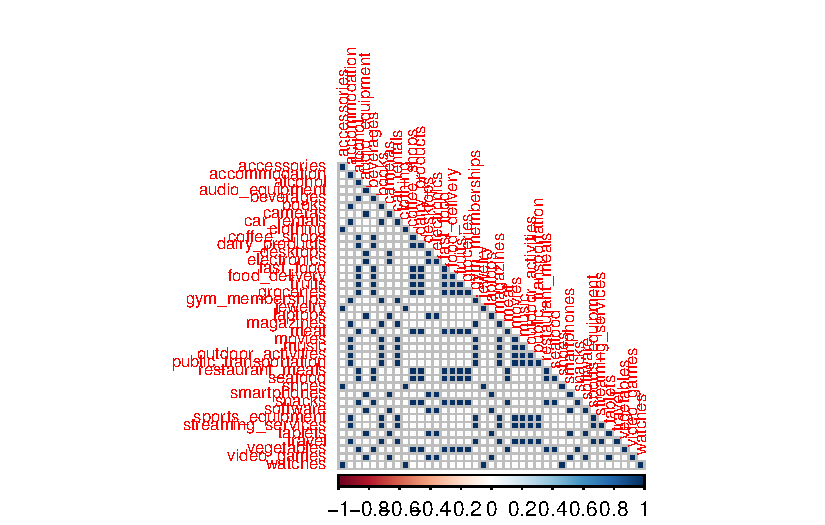
\includegraphics{hw6_files/figure-pdf/unnamed-chunk-3-1.pdf}

\begin{center}\rule{0.5\linewidth}{0.5pt}\end{center}

1.3 (5 points)

Run a linear regression model to predict the \texttt{income} variable
using the remaining predictors. Interpret the coefficients and summarize
your results.

\begin{Shaded}
\begin{Highlighting}[]
\NormalTok{model }\OtherTok{\textless{}{-}} \FunctionTok{lm}\NormalTok{(income }\SpecialCharTok{\textasciitilde{}}\NormalTok{ ., }\AttributeTok{data =}\NormalTok{ df)}
\FunctionTok{summary}\NormalTok{(model)}
\end{Highlighting}
\end{Shaded}

\begin{verbatim}

Call:
lm(formula = income ~ ., data = df)

Residuals:
    Min      1Q  Median      3Q     Max 
-8.6875 -1.6569  0.0427  1.6633  9.5623 

Coefficients:
                       Estimate Std. Error t value Pr(>|t|)    
(Intercept)           -0.077509   0.121730  -0.637 0.524330    
accessories            0.299876   0.031786   9.434  < 2e-16 ***
accommodation          0.113632   0.031262   3.635 0.000281 ***
alcohol               -0.005958   0.033266  -0.179 0.857873    
audio_equipment        0.602004   0.033483  17.979  < 2e-16 ***
beverages              0.043335   0.034111   1.270 0.204000    
books                  0.070530   0.033238   2.122 0.033892 *  
cameras                0.461827   0.033572  13.756  < 2e-16 ***
car_rentals            0.124875   0.032809   3.806 0.000143 ***
clothing               0.504228   0.026055  19.352  < 2e-16 ***
coffee_shops           0.048839   0.034909   1.399 0.161864    
dairy_products         0.024548   0.032715   0.750 0.453082    
desktops               0.391673   0.033393  11.729  < 2e-16 ***
electronics            1.079627   0.030035  35.946  < 2e-16 ***
fast_food              0.077531   0.033014   2.348 0.018893 *  
food_delivery         -0.004903   0.034257  -0.143 0.886188    
fruits                 0.059089   0.033321   1.773 0.076237 .  
groceries              0.077694   0.031601   2.459 0.013981 *  
gym_memberships        0.141168   0.033410   4.225 2.43e-05 ***
jewelry                0.213726   0.032834   6.509 8.30e-11 ***
laptops                0.594328   0.032548  18.260  < 2e-16 ***
magazines              0.080762   0.033694   2.397 0.016571 *  
meat                   0.081262   0.032367   2.511 0.012083 *  
movies                 0.110296   0.033326   3.310 0.000941 ***
music                  0.159925   0.033398   4.788 1.73e-06 ***
outdoor_activities     0.087846   0.032356   2.715 0.006651 ** 
public_transportation  0.061138   0.033022   1.851 0.064169 .  
restaurant_meals       0.066129   0.033225   1.990 0.046611 *  
seafood                0.061318   0.033786   1.815 0.069596 .  
shoes                  0.463185   0.029613  15.641  < 2e-16 ***
smartphones            0.780150   0.031538  24.737  < 2e-16 ***
snacks                 0.007464   0.033229   0.225 0.822290    
software               0.408500   0.034102  11.979  < 2e-16 ***
sports_equipment       0.033328   0.033969   0.981 0.326574    
streaming_services     0.150614   0.031902   4.721 2.41e-06 ***
tablets                0.637266   0.033133  19.234  < 2e-16 ***
travel                 0.129161   0.031457   4.106 4.09e-05 ***
vegetables            -0.066111   0.033162  -1.994 0.046257 *  
video_games            0.863309   0.031392  27.501  < 2e-16 ***
watches                0.145853   0.033467   4.358 1.34e-05 ***
---
Signif. codes:  0 '***' 0.001 '**' 0.01 '*' 0.05 '.' 0.1 ' ' 1

Residual standard error: 2.434 on 4960 degrees of freedom
Multiple R-squared:  0.9999,    Adjusted R-squared:  0.9999 
F-statistic: 1.834e+06 on 39 and 4960 DF,  p-value: < 2.2e-16
\end{verbatim}

\begin{center}\rule{0.5\linewidth}{0.5pt}\end{center}

1.3 (5 points)

Diagnose the model using the \texttt{vif()} function. What do you
observe? What does this mean for the model?

\begin{Shaded}
\begin{Highlighting}[]
\NormalTok{vif\_values }\OtherTok{\textless{}{-}} \FunctionTok{vif}\NormalTok{(model)}
\FunctionTok{print}\NormalTok{(vif\_values)}
\end{Highlighting}
\end{Shaded}

\begin{verbatim}
          accessories         accommodation               alcohol 
            152.06821             681.15504             387.23376 
      audio_equipment             beverages                 books 
           1755.56441             914.69186             192.91781 
              cameras           car_rentals              clothing 
            785.43147             423.55906             282.25143 
         coffee_shops        dairy_products              desktops 
            425.39644            2336.74847             776.75697 
          electronics             fast_food         food_delivery 
           3927.16511            1519.85171             921.68162 
               fruits             groceries       gym_memberships 
           1550.05678            3136.80325             438.30224 
              jewelry               laptops             magazines 
             72.38215            1658.76990             198.53619 
                 meat                movies                 music 
           2284.43676             437.28082             437.03990 
   outdoor_activities public_transportation      restaurant_meals 
            411.17302             427.77815            1540.26240 
              seafood                 shoes           smartphones 
           1594.08027             233.33301            2772.27822 
               snacks              software      sports_equipment 
            868.24282             810.28919             201.00255 
   streaming_services               tablets                travel 
            709.25592            1718.78339             690.69616 
           vegetables           video_games               watches 
           1536.40686            2745.64421              75.56457 
\end{verbatim}

\begin{center}\rule{0.5\linewidth}{0.5pt}\end{center}

1.4 (5 points)

Perform PCA using the \texttt{princomp} function in R. Print the summary
of the PCA object.

\begin{Shaded}
\begin{Highlighting}[]
\NormalTok{pca }\OtherTok{\textless{}{-}} \FunctionTok{princomp}\NormalTok{(df }\SpecialCharTok{\%\textgreater{}\%} \FunctionTok{select}\NormalTok{(}\SpecialCharTok{{-}}\NormalTok{income), }\AttributeTok{cor =} \ConstantTok{TRUE}\NormalTok{)}
\FunctionTok{summary}\NormalTok{(pca)}
\end{Highlighting}
\end{Shaded}

\begin{verbatim}
Importance of components:
                          Comp.1    Comp.2    Comp.3    Comp.4       Comp.5
Standard deviation     3.6201099 3.4479976 2.9939875 2.2288727 0.1125697569
Proportion of Variance 0.3360307 0.3048381 0.2298452 0.1273814 0.0003249218
Cumulative Proportion  0.3360307 0.6408688 0.8707140 0.9980954 0.9984202743
                             Comp.6       Comp.7       Comp.8       Comp.9
Standard deviation     0.0960605322 0.0708312069 0.0691539249 0.0670242037
Proportion of Variance 0.0002366058 0.0001286426 0.0001226222 0.0001151857
Cumulative Proportion  0.9986568801 0.9987855227 0.9989081448 0.9990233306
                            Comp.10      Comp.11      Comp.12      Comp.13
Standard deviation     0.0653196274 5.099363e-02 0.0498072940 4.762347e-02
Proportion of Variance 0.0001094014 6.667565e-05 0.0000636094 5.815371e-05
Cumulative Proportion  0.9991327320 9.991994e-01 0.9992630170 9.993212e-01
                            Comp.14      Comp.15      Comp.16      Comp.17
Standard deviation     0.0469865879 4.611213e-02 0.0459026903 4.552808e-02
Proportion of Variance 0.0000566087 5.452125e-05 0.0000540271 5.314888e-05
Cumulative Proportion  0.9993777794 9.994323e-01 0.9994863278 9.995395e-01
                            Comp.18      Comp.19      Comp.20      Comp.21
Standard deviation     4.516751e-02 3.944038e-02 0.0358645643 3.505209e-02
Proportion of Variance 5.231037e-05 3.988573e-05 0.0000329812 3.150383e-05
Cumulative Proportion  9.995918e-01 9.996317e-01 0.9996646540 9.996962e-01
                            Comp.22      Comp.23      Comp.24      Comp.25
Standard deviation     3.460809e-02 3.435268e-02 3.297822e-02 3.240319e-02
Proportion of Variance 3.071076e-05 3.025915e-05 2.788623e-05 2.692223e-05
Cumulative Proportion  9.997269e-01 9.997571e-01 9.997850e-01 9.998119e-01
                            Comp.26      Comp.27      Comp.28      Comp.29
Standard deviation     3.135574e-02 2.976920e-02 2.508623e-02 2.460025e-02
Proportion of Variance 2.520981e-05 2.272321e-05 1.613638e-05 1.551723e-05
Cumulative Proportion  9.998371e-01 9.998599e-01 9.998760e-01 9.998915e-01
                            Comp.30      Comp.31      Comp.32      Comp.33
Standard deviation     2.426600e-02 2.374599e-02 2.334190e-02 2.283049e-02
Proportion of Variance 1.509843e-05 1.445825e-05 1.397036e-05 1.336491e-05
Cumulative Proportion  9.999066e-01 9.999211e-01 9.999350e-01 9.999484e-01
                            Comp.34      Comp.35      Comp.36      Comp.37
Standard deviation     2.119139e-02 1.968544e-02 1.937808e-02 1.742835e-02
Proportion of Variance 1.151475e-05 9.936319e-06 9.628464e-06 7.788395e-06
Cumulative Proportion  9.999599e-01 9.999699e-01 9.999795e-01 9.999873e-01
                            Comp.38      Comp.39
Standard deviation     1.677847e-02 1.464440e-02
Proportion of Variance 7.218385e-06 5.498931e-06
Cumulative Proportion  9.999945e-01 1.000000e+00
\end{verbatim}

\begin{center}\rule{0.5\linewidth}{0.5pt}\end{center}

1.5 (5 points)

Make a screeplot of the proportion of variance explained by each
principal component. How many principal components would you choose to
keep? Why?

\begin{Shaded}
\begin{Highlighting}[]
\NormalTok{scree\_plot }\OtherTok{\textless{}{-}} \FunctionTok{qplot}\NormalTok{(}\FunctionTok{c}\NormalTok{(}\DecValTok{1}\SpecialCharTok{:}\FunctionTok{length}\NormalTok{(pca}\SpecialCharTok{$}\NormalTok{sdev)), pca}\SpecialCharTok{$}\NormalTok{sdev}\SpecialCharTok{\^{}}\DecValTok{2}\SpecialCharTok{/}\FunctionTok{sum}\NormalTok{(pca}\SpecialCharTok{$}\NormalTok{sdev}\SpecialCharTok{\^{}}\DecValTok{2}\NormalTok{), }
                    \AttributeTok{xlab =} \StringTok{"Principal Component"}\NormalTok{, }
                    \AttributeTok{ylab =} \StringTok{"Proportion of Variance Explained"}\NormalTok{) }\SpecialCharTok{+}
  \FunctionTok{geom\_line}\NormalTok{() }\SpecialCharTok{+}
  \FunctionTok{theme\_bw}\NormalTok{()}
\end{Highlighting}
\end{Shaded}

\begin{verbatim}
Warning: `qplot()` was deprecated in ggplot2 3.4.0.
\end{verbatim}

\begin{Shaded}
\begin{Highlighting}[]
\NormalTok{scree\_plot}
\end{Highlighting}
\end{Shaded}

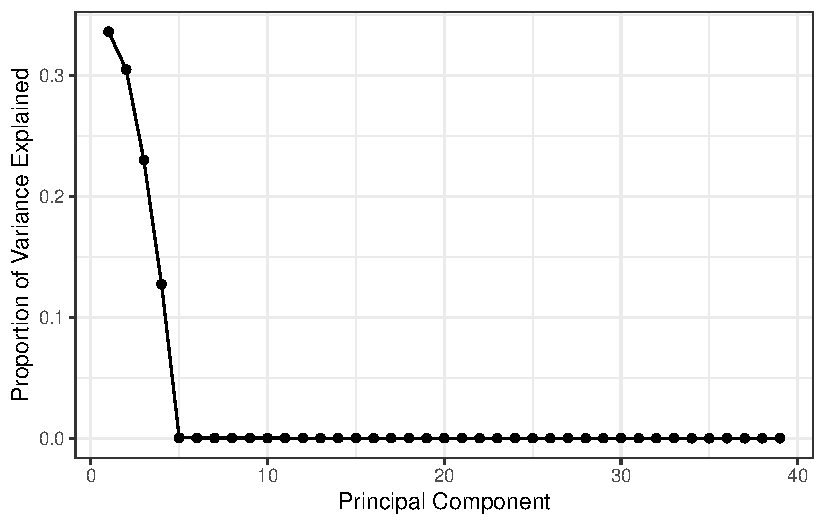
\includegraphics{hw6_files/figure-pdf/unnamed-chunk-7-1.pdf}

1.6 (5 points)

By setting any factor loadings below \(0.2\) to \(0\), summarize the
factor loadings for the principal components that you chose to keep.

\begin{Shaded}
\begin{Highlighting}[]
\NormalTok{num\_components }\OtherTok{\textless{}{-}} \DecValTok{3}

\NormalTok{clean\_loadings }\OtherTok{\textless{}{-}}\NormalTok{ pca}\SpecialCharTok{$}\NormalTok{loadings[, }\DecValTok{1}\SpecialCharTok{:}\NormalTok{num\_components]}
\NormalTok{clean\_loadings[}\FunctionTok{abs}\NormalTok{(clean\_loadings) }\SpecialCharTok{\textless{}} \FloatTok{0.2}\NormalTok{] }\OtherTok{\textless{}{-}} \DecValTok{0}

\NormalTok{loadings\_data }\OtherTok{\textless{}{-}} \FunctionTok{melt}\NormalTok{(clean\_loadings)}
\FunctionTok{colnames}\NormalTok{(loadings\_data) }\OtherTok{\textless{}{-}} \FunctionTok{c}\NormalTok{(}\StringTok{"Variable"}\NormalTok{, }\StringTok{"Component"}\NormalTok{, }\StringTok{"Loading"}\NormalTok{)}

\NormalTok{loadings\_plot }\OtherTok{\textless{}{-}} \FunctionTok{ggplot}\NormalTok{(loadings\_data, }\FunctionTok{aes}\NormalTok{(Variable, Component, }\AttributeTok{fill =}\NormalTok{ Loading)) }\SpecialCharTok{+}
  \FunctionTok{geom\_tile}\NormalTok{() }\SpecialCharTok{+}
  \FunctionTok{scale\_fill\_gradient2}\NormalTok{(}\AttributeTok{low =} \StringTok{"blue"}\NormalTok{, }\AttributeTok{mid =} \StringTok{"white"}\NormalTok{, }\AttributeTok{high =} \StringTok{"red"}\NormalTok{, }
                       \AttributeTok{midpoint =} \DecValTok{0}\NormalTok{, }\AttributeTok{limit =} \FunctionTok{c}\NormalTok{(}\SpecialCharTok{{-}}\DecValTok{1}\NormalTok{, }\DecValTok{1}\NormalTok{)) }\SpecialCharTok{+}
  \FunctionTok{labs}\NormalTok{(}\AttributeTok{title =} \StringTok{"Factor Loadings"}\NormalTok{, }\AttributeTok{x =} \StringTok{"Variable"}\NormalTok{, }\AttributeTok{y =} \StringTok{"Component"}\NormalTok{) }\SpecialCharTok{+}
  \FunctionTok{theme\_bw}\NormalTok{()}

\NormalTok{loadings\_plot}
\end{Highlighting}
\end{Shaded}

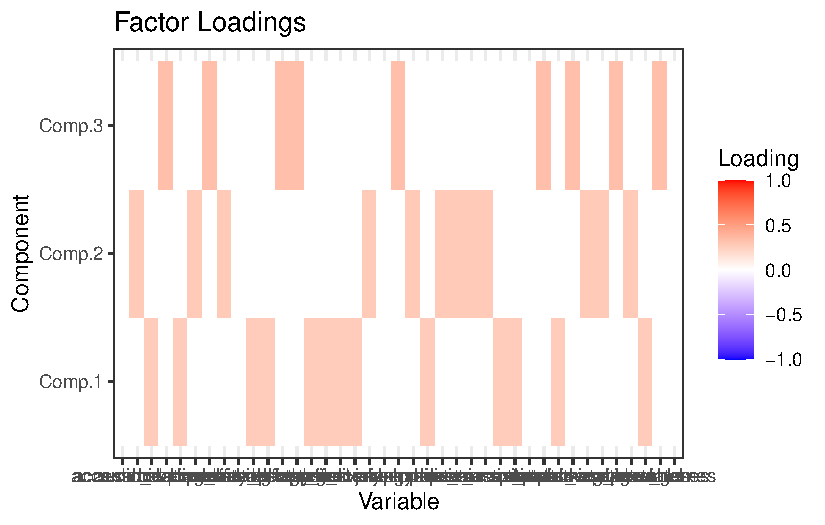
\includegraphics{hw6_files/figure-pdf/unnamed-chunk-8-1.pdf}

Visualize the factor loadings.

\begin{Shaded}
\begin{Highlighting}[]
\NormalTok{df\_pca }\OtherTok{\textless{}{-}} \FunctionTok{cbind}\NormalTok{(df}\SpecialCharTok{$}\NormalTok{income, pca}\SpecialCharTok{$}\NormalTok{scores[, }\DecValTok{1}\SpecialCharTok{:}\NormalTok{num\_components])}
\FunctionTok{colnames}\NormalTok{(df\_pca) }\OtherTok{\textless{}{-}} \FunctionTok{c}\NormalTok{(}\StringTok{"income"}\NormalTok{, }\FunctionTok{paste0}\NormalTok{(}\StringTok{"PC"}\NormalTok{, }\DecValTok{1}\SpecialCharTok{:}\NormalTok{num\_components))}
\end{Highlighting}
\end{Shaded}

\begin{center}\rule{0.5\linewidth}{0.5pt}\end{center}

1.7 (15 points)

Based on the factor loadings, what do you think the principal components
represent?

Provide an interpreation for each principal component you chose to keep.

\begin{center}\rule{0.5\linewidth}{0.5pt}\end{center}

1.8 (10 points)

Create a new data frame with the original response variable
\texttt{income} and the principal components you chose to keep. Call
this data frame \texttt{df\_pca}.

\begin{Shaded}
\begin{Highlighting}[]
\NormalTok{num\_components }\OtherTok{\textless{}{-}} \DecValTok{3}  
\NormalTok{df\_pca }\OtherTok{\textless{}{-}} \FunctionTok{cbind}\NormalTok{(df}\SpecialCharTok{$}\NormalTok{income, pca}\SpecialCharTok{$}\NormalTok{scores[, }\DecValTok{1}\SpecialCharTok{:}\NormalTok{num\_components])}
\FunctionTok{colnames}\NormalTok{(df\_pca) }\OtherTok{\textless{}{-}} \FunctionTok{c}\NormalTok{(}\StringTok{"income"}\NormalTok{, }\FunctionTok{paste0}\NormalTok{(}\StringTok{"PC"}\NormalTok{, }\DecValTok{1}\SpecialCharTok{:}\NormalTok{num\_components))}
\end{Highlighting}
\end{Shaded}

Fit a regression model to predict the \texttt{income} variable using the
principal components you chose to keep. Interpret the coefficients and
summarize your results.

\begin{Shaded}
\begin{Highlighting}[]
\NormalTok{num\_components }\OtherTok{\textless{}{-}} \DecValTok{3}
\NormalTok{df\_pca }\OtherTok{\textless{}{-}} \FunctionTok{cbind}\NormalTok{(df}\SpecialCharTok{$}\NormalTok{income, pca}\SpecialCharTok{$}\NormalTok{scores[, }\DecValTok{1}\SpecialCharTok{:}\NormalTok{num\_components])}
\FunctionTok{colnames}\NormalTok{(df\_pca) }\OtherTok{\textless{}{-}} \FunctionTok{c}\NormalTok{(}\StringTok{"income"}\NormalTok{, }\FunctionTok{paste0}\NormalTok{(}\StringTok{"PC"}\NormalTok{, }\DecValTok{1}\SpecialCharTok{:}\NormalTok{num\_components))}

\NormalTok{df\_pca }\OtherTok{\textless{}{-}} \FunctionTok{as.data.frame}\NormalTok{(df\_pca)}

\NormalTok{model\_pca }\OtherTok{\textless{}{-}} \FunctionTok{lm}\NormalTok{(income }\SpecialCharTok{\textasciitilde{}}\NormalTok{ ., }\AttributeTok{data =}\NormalTok{ df\_pca)}
\FunctionTok{summary}\NormalTok{(model\_pca)}
\end{Highlighting}
\end{Shaded}

\begin{verbatim}

Call:
lm(formula = income ~ ., data = df_pca)

Residuals:
    Min      1Q  Median      3Q     Max 
-44.345 -18.599  -0.293  18.730  47.846 

Coefficients:
             Estimate Std. Error t value Pr(>|t|)    
(Intercept) 628.17783    0.30371  2068.4   <2e-16 ***
PC1          13.33571    0.08390   159.0   <2e-16 ***
PC2          -1.16303    0.08808   -13.2   <2e-16 ***
PC3          95.58547    0.10144   942.3   <2e-16 ***
---
Signif. codes:  0 '***' 0.001 '**' 0.01 '*' 0.05 '.' 0.1 ' ' 1

Residual standard error: 21.48 on 4996 degrees of freedom
Multiple R-squared:  0.9946,    Adjusted R-squared:  0.9946 
F-statistic: 3.044e+05 on 3 and 4996 DF,  p-value: < 2.2e-16
\end{verbatim}

Compare the results of the regression model in 1.3 and 1.9. What do you
observe? What does this mean for the model?

\begin{Shaded}
\begin{Highlighting}[]
\FunctionTok{summary}\NormalTok{(model)  }
\end{Highlighting}
\end{Shaded}

\begin{verbatim}

Call:
lm(formula = income ~ ., data = df)

Residuals:
    Min      1Q  Median      3Q     Max 
-8.6875 -1.6569  0.0427  1.6633  9.5623 

Coefficients:
                       Estimate Std. Error t value Pr(>|t|)    
(Intercept)           -0.077509   0.121730  -0.637 0.524330    
accessories            0.299876   0.031786   9.434  < 2e-16 ***
accommodation          0.113632   0.031262   3.635 0.000281 ***
alcohol               -0.005958   0.033266  -0.179 0.857873    
audio_equipment        0.602004   0.033483  17.979  < 2e-16 ***
beverages              0.043335   0.034111   1.270 0.204000    
books                  0.070530   0.033238   2.122 0.033892 *  
cameras                0.461827   0.033572  13.756  < 2e-16 ***
car_rentals            0.124875   0.032809   3.806 0.000143 ***
clothing               0.504228   0.026055  19.352  < 2e-16 ***
coffee_shops           0.048839   0.034909   1.399 0.161864    
dairy_products         0.024548   0.032715   0.750 0.453082    
desktops               0.391673   0.033393  11.729  < 2e-16 ***
electronics            1.079627   0.030035  35.946  < 2e-16 ***
fast_food              0.077531   0.033014   2.348 0.018893 *  
food_delivery         -0.004903   0.034257  -0.143 0.886188    
fruits                 0.059089   0.033321   1.773 0.076237 .  
groceries              0.077694   0.031601   2.459 0.013981 *  
gym_memberships        0.141168   0.033410   4.225 2.43e-05 ***
jewelry                0.213726   0.032834   6.509 8.30e-11 ***
laptops                0.594328   0.032548  18.260  < 2e-16 ***
magazines              0.080762   0.033694   2.397 0.016571 *  
meat                   0.081262   0.032367   2.511 0.012083 *  
movies                 0.110296   0.033326   3.310 0.000941 ***
music                  0.159925   0.033398   4.788 1.73e-06 ***
outdoor_activities     0.087846   0.032356   2.715 0.006651 ** 
public_transportation  0.061138   0.033022   1.851 0.064169 .  
restaurant_meals       0.066129   0.033225   1.990 0.046611 *  
seafood                0.061318   0.033786   1.815 0.069596 .  
shoes                  0.463185   0.029613  15.641  < 2e-16 ***
smartphones            0.780150   0.031538  24.737  < 2e-16 ***
snacks                 0.007464   0.033229   0.225 0.822290    
software               0.408500   0.034102  11.979  < 2e-16 ***
sports_equipment       0.033328   0.033969   0.981 0.326574    
streaming_services     0.150614   0.031902   4.721 2.41e-06 ***
tablets                0.637266   0.033133  19.234  < 2e-16 ***
travel                 0.129161   0.031457   4.106 4.09e-05 ***
vegetables            -0.066111   0.033162  -1.994 0.046257 *  
video_games            0.863309   0.031392  27.501  < 2e-16 ***
watches                0.145853   0.033467   4.358 1.34e-05 ***
---
Signif. codes:  0 '***' 0.001 '**' 0.01 '*' 0.05 '.' 0.1 ' ' 1

Residual standard error: 2.434 on 4960 degrees of freedom
Multiple R-squared:  0.9999,    Adjusted R-squared:  0.9999 
F-statistic: 1.834e+06 on 39 and 4960 DF,  p-value: < 2.2e-16
\end{verbatim}

\begin{Shaded}
\begin{Highlighting}[]
\FunctionTok{summary}\NormalTok{(model\_pca)  }
\end{Highlighting}
\end{Shaded}

\begin{verbatim}

Call:
lm(formula = income ~ ., data = df_pca)

Residuals:
    Min      1Q  Median      3Q     Max 
-44.345 -18.599  -0.293  18.730  47.846 

Coefficients:
             Estimate Std. Error t value Pr(>|t|)    
(Intercept) 628.17783    0.30371  2068.4   <2e-16 ***
PC1          13.33571    0.08390   159.0   <2e-16 ***
PC2          -1.16303    0.08808   -13.2   <2e-16 ***
PC3          95.58547    0.10144   942.3   <2e-16 ***
---
Signif. codes:  0 '***' 0.001 '**' 0.01 '*' 0.05 '.' 0.1 ' ' 1

Residual standard error: 21.48 on 4996 degrees of freedom
Multiple R-squared:  0.9946,    Adjusted R-squared:  0.9946 
F-statistic: 3.044e+05 on 3 and 4996 DF,  p-value: < 2.2e-16
\end{verbatim}

\begin{Shaded}
\begin{Highlighting}[]
\NormalTok{metrics }\OtherTok{\textless{}{-}} \FunctionTok{rbind}\NormalTok{(}
  \FunctionTok{data.frame}\NormalTok{(}\AttributeTok{Model =} \StringTok{"Original"}\NormalTok{, }\AttributeTok{RMSE =} \FunctionTok{sqrt}\NormalTok{(}\FunctionTok{mean}\NormalTok{(model}\SpecialCharTok{$}\NormalTok{residuals}\SpecialCharTok{\^{}}\DecValTok{2}\NormalTok{)), }\AttributeTok{R2 =} \FunctionTok{summary}\NormalTok{(model)}\SpecialCharTok{$}\NormalTok{r.squared),}
  \FunctionTok{data.frame}\NormalTok{(}\AttributeTok{Model =} \StringTok{"PCA"}\NormalTok{, }\AttributeTok{RMSE =} \FunctionTok{sqrt}\NormalTok{(}\FunctionTok{mean}\NormalTok{(model\_pca}\SpecialCharTok{$}\NormalTok{residuals}\SpecialCharTok{\^{}}\DecValTok{2}\NormalTok{)), }\AttributeTok{R2 =} \FunctionTok{summary}\NormalTok{(model\_pca)}\SpecialCharTok{$}\NormalTok{r.squared)}
\NormalTok{)}

\FunctionTok{print}\NormalTok{(metrics)}
\end{Highlighting}
\end{Shaded}

\begin{verbatim}
     Model      RMSE        R2
1 Original  2.423783 0.9999306
2      PCA 21.466895 0.9945598
\end{verbatim}

\begin{center}\rule{0.5\linewidth}{0.5pt}\end{center}

1.10 (10 points)

Based on your interpretation of the principal components from Question
1.7, provide an interpretation of the regression model in Question 1.9.

\begin{center}\rule{0.5\linewidth}{0.5pt}\end{center}

\pagebreak

---

\begin{tcolorbox}[enhanced jigsaw, leftrule=.75mm, rightrule=.15mm, left=2mm, colframe=quarto-callout-note-color-frame, bottomtitle=1mm, colbacktitle=quarto-callout-note-color!10!white, titlerule=0mm, breakable, opacitybacktitle=0.6, coltitle=black, arc=.35mm, colback=white, title=\textcolor{quarto-callout-note-color}{\faInfo}\hspace{0.5em}{Session Information}, toptitle=1mm, toprule=.15mm, bottomrule=.15mm, opacityback=0]

Print your \texttt{R} session information using the following command

\begin{Shaded}
\begin{Highlighting}[]
\FunctionTok{sessionInfo}\NormalTok{()}
\end{Highlighting}
\end{Shaded}

\begin{verbatim}
R version 4.3.3 (2024-02-29 ucrt)
Platform: x86_64-w64-mingw32/x64 (64-bit)
Running under: Windows 11 x64 (build 22631)

Matrix products: default


locale:
[1] LC_COLLATE=English_United States.utf8 
[2] LC_CTYPE=English_United States.utf8   
[3] LC_MONETARY=English_United States.utf8
[4] LC_NUMERIC=C                          
[5] LC_TIME=English_United States.utf8    

time zone: America/New_York
tzcode source: internal

attached base packages:
[1] stats     graphics  grDevices datasets  utils     methods   base     

other attached packages:
 [1] reshape2_1.4.4 ggplot2_3.5.0  janitor_2.2.0  car_3.1-2      carData_3.0-5 
 [6] corrplot_0.92  magrittr_2.0.3 broom_1.0.5    purrr_1.0.2    tidyr_1.3.1   
[11] readr_2.1.5    dplyr_1.1.4    tibble_3.2.1  

loaded via a namespace (and not attached):
 [1] utf8_1.2.4        generics_0.1.3    renv_1.0.3        stringi_1.8.3    
 [5] hms_1.1.3         digest_0.6.35     evaluate_0.23     grid_4.3.3       
 [9] timechange_0.3.0  fastmap_1.1.1     plyr_1.8.9        jsonlite_1.8.8   
[13] backports_1.4.1   tinytex_0.50      fansi_1.0.6       scales_1.3.0     
[17] codetools_0.2-19  abind_1.4-5       cli_3.6.2         crayon_1.5.2     
[21] rlang_1.1.3       bit64_4.0.5       munsell_0.5.1     withr_3.0.0      
[25] yaml_2.3.8        parallel_4.3.3    tools_4.3.3       tzdb_0.4.0       
[29] colorspace_2.1-0  vctrs_0.6.5       R6_2.5.1          lifecycle_1.0.4  
[33] lubridate_1.9.3   snakecase_0.11.1  stringr_1.5.1     bit_4.0.5        
[37] vroom_1.6.5       pkgconfig_2.0.3   pillar_1.9.0      gtable_0.3.4     
[41] glue_1.7.0        Rcpp_1.0.12       xfun_0.43         tidyselect_1.2.1 
[45] knitr_1.46        farver_2.1.1      htmltools_0.5.8.1 labeling_0.4.3   
[49] rmarkdown_2.26    compiler_4.3.3   
\end{verbatim}

\end{tcolorbox}



\end{document}
